\section{Preliminaries}
\label{sec:preliminaries}

\subsection{Stochastic Models}
\label{sec:Stochastic Models}

\begin{definition}[Markov chains]
\label{def:Markov Chains}
A Markov Chain $\mathcal{C}$ is a tuple $(Q, \delta)$ where Q is a finite set of states and 
$\delta: Q \rightarrow \mathbb{D}(Q)$ is a probabilistic transition function, where 
$\mathbb{D}(Q)$ is the set of all probabilistic distribution on a finite set $Q$. A probabilistic distribution on 
$Q$, is a function $f: Q\rightarrow\mathbb{Q}_{\geq0}$ such that $\sum_{q\in Q}f(q)=1$. 
\end{definition}

\noindent
A non-empty finite word $\varrho = p_1p_2...p_n$ over $Q$ is defined as a run of Markov Chain. 
The probability of the run is $\prod_{0\leq i < n}\delta(p_i,p_{i+1})$. 
$\varrho$ reaches $q$, if $q = p_i$ for some $0\leq i\leq n$. 
\newline
\\
The probability of eventually reaching a set of state $T\subseteq Q$ 
in $\mathcal{C}$ starting from $q_0$ can be denoted as $\mathbb{P}^{q_0}_\mathcal{C}[\lozenge T]$. $\lozenge T$ is 
equivalent to $Q\bigcup T$, Q until T. Since not necessary every state in Q is reached before T, 
a set of states $S\subseteq Q$ is defined, where the path until T only consists of these states.
The probability $\mathbb{P}^{q_0}_\mathcal{C}[S\bigcup T]$. If $q_0 \in T$, 
the probability is 1. Otherwise, the probability is calculated as follows: 
\begin{align*}
    \sum\biggl\{ \prod_{0\leq i< n}\delta(q_i,q_{i+1}) ~|~ q_0...q_{n-1}\in (S~\backslash~ T) ~\&~ q_n 
    \in T\ \text{ for } n\geq 1\biggr\}.
\end{align*}

\noindent
If there exists a set $U\subseteq Q$, where all runs from $q_0$ to $T$ reaches, the probability of 
$\mathbb{P}^{q_0}_\mathcal{C}[\lozenge T]$ can be reduced to the following lemma:  

\begin{lemma}
\label{lemma 1}
Consider a Markov Chain $\mathcal{C}=(Q,\delta)$ set of states $U,T\subseteq Q$, and a state $q_0\in Q\backslash U$. 
If $\mathbb{P}^{q_0}_\mathcal{C}[(Q\backslash U)\bigcup T]=0$, then 
\begin{align*}
    \mathbb{P}^{q_0}_\mathcal{C}[\lozenge T] = \sum_{u\in U}\mathbb{P}^{q_0}_\mathcal{C}[(Q\backslash U) \bigcup u]
    \mathbb{P}^{q_0}_\mathcal{C}[\lozenge T]
\end{align*}
\end{lemma}


\begin{definition}[Markov decision processes]
\label{Markov decision processes}
A (finite and discrete-time) Markov decision processes, MDP, $\mathcal{M}$, is a tuple $(Q,A,\delta,T)$ 
where Q is a finite set of states, A a finite set of actions, $\delta: Q \times A \rightarrow \mathbb{D}(Q)$ 
a probabilistic transition function, and $T\subseteq Q$ a set of target state.
\end{definition}

\noindent
The notation for the probability of the state p reaching q with the action a, $\delta(p,a)(q)$ will be changed to 
$\delta(q|p,a)$ for convenience.

\begin{definition}[Strategies]
\label{Strategies}
A (memoryless deterministic) strategy $\sigma$ in an MDP M = $(Q,A,\delta,T)$ is a function $\sigma: Q\rightarrow A$.
\end{definition}

\noindent
\textit{From MDPs to Chains} An MDP $\mathcal{M} = (Q,A,\delta,T)$ and a Markov Chain $M^\sigma = (Q, \mu)$, 
where a strategy $\sigma$ is applied on. $\mu$ is defined as follows: $\mu(q)=\delta(q,\sigma(q))$ for all $q\in Q$.
The probability of q, $\mu(q)$, is the same as $\delta(q,\sigma(q))$, where $\sigma(q)$ gives the action assigned to q. 
\begin{figure}[htb]
	\begin{center}
		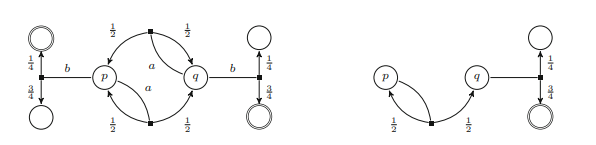
\includegraphics[width=1\linewidth]{pictures/strategies.png}
	\end{center}
	\caption{MDP on the left and 
    on the right a Markov chain induced by the left MDP. \cite{10.1007/978-3-319-89366-2_20}}
	\label{fig:strategies}
\end{figure}

\noindent
The MDP on the left in Figure \ref{fig:strategies} has the actions $\{a, b\}$. The states are shown as circles,
the states with double circles are target states, the squares are distributions. 
The arrows from states to distributions shows which action is used and the arrows from distributions to states are probabilities.
\newline
\\
The strategy $\sigma$ for the right Markov chain maps as follows: $\{p \mapsto a, q \mapsto b\}$ i.e. $\sigma(p) = a, \sigma(q) = b$.
Since the strategy $\sigma$ is applied on the Markov chain, the arrows with actions are removed. 
With the Markov chain, the easier probability to calculate would be $\mathbb{P}^{q}_{\mathcal{M}^\sigma}[\lozenge T] = \frac{3}{4}$.
The probability is written on the arrow from the distributions, after the state q, to the target state.

\subsection{Reachability Games Against Nature}
It is often difficult to determine the probability $\mathbb{P}^{q_0}_\mathcal{C}[\lozenge T]$. 
That is why families of MDP with the same support, where the probabilities are abstracted, will be considered. 
The focus is directed to the underlying directed graph from the MDP, where a game against nature is played on.
Given an MDP $\mathcal{M}=(Q,A,\delta,T)$, the underlying directed graph $\mathcal{G}_\mathcal{M}=(V,E)$ with 
$V:= Q\cup (Q\times A)$ and $E:={(q,\langle q,a\rangle)\in Q\times (Q\times A)}\cup{(\langle p,a\rangle,q)~|~\delta(q|p,a)>0}$.
To simplify, the vertex set consists of state vertices and state-action vertices. 
The edges consist of state to state-action edges $(q,\langle q,a\rangle)$ 
state-action to next state edges $(\langle p,a\rangle,q)$, where $\delta(q|p,a)>0$. 
\textit{Nature} controls the vertices $Q\times A$ in $\mathcal{G}_\mathcal{M}$. The game is played on the following arena. 

\begin{definition}[Target Arena]
\label{def:target arena}
A target arena is a tuple $\mathcal{A}:= (V,V_P,E,T)$ with the bipartite directed graph $(V_P,V_N,E)$, and $T\subseteq V_P$. 
$V_N:= V\backslash V_P$ and for all $u\in V_N$, $uE \neq \emptyset$ with $uE$ being the set of successors of $u$. 
    
\end{definition}

\noindent
In this game \textit{Nature} controls the vertices $V_N$ and \textit{Protagonist} controls the vertices $V_P$. 
In order to make the arena into an MDP, a family of probability distributions $\mu$ using the arena $\mathcal{A}$ will be applied to the MDP.
Let the MDP $\mathcal{A}_\mu$ be defined as follows: $\mathcal{A}_\mu = (Q, A, \delta, T)$ with $\mu =(\mu_u \in \mathbb{D}(uE))_{u\in V_N},~ 
Q=V_P \uplus\{\perp\},~ A=V_N$. $\delta(q|p,a)$ is $\mu_a(q)$ if $(p,a)(a,q)\in E$ and otherwise 0. 
For all $p\in V_P\cup \{\perp\}$ and $a\in A$, $\delta(\perp|p,a)= 1$, if $(p,a) \not\in E$.
\newline
\\
The value of the vertex on the target arena $\mathcal{A}$ differentiate between vertices from $V_P$ and $ V_N$. 
The maximal reachability probability value of both are defined with respect of full-support probability distributions $\mu$. 
For $v\in V_P$ the value is defined as $Val^\mu(v):= max_\sigma \mathbb{P}^v_{\mathcal{A}^\sigma_\mu}[\lozenge T]$. 
That means the max reachability probability value of a vertex from the Protagonist is 
the maximal probability of reaching T from v in $\mathcal{A}^\sigma_\mu$, 
the target arena induced with the strategy $\sigma$ and the probability distribution $\mu$. 
For $u\in V_N$ the value is defined as $Val^\mu(u):=\sum\{\mu_u(v)Val^\mu(v)~|~v\in uE\}$, with $Val^\mu(v)$ defined above, 
since the arena is a bipartite directed graph.


